\documentclass[10pt]{article}
\usepackage{itcep, stmaryrd, tikz, pgflibraryplotmarks, multicol}
\usepackage[margin=1in, nohead, pdftex]{geometry}
\usepackage{MnSymbol,wasysym}
\usepackage{hyperref}
\usepackage{enumitem}

\topmargin -0.2in
\pagestyle{empty}
\singlespacing
\let\oldhat\hat
\renewcommand{\vec}[1]{\mathbf{#1}}
\renewcommand{\hat}[1]{\oldhat{\mathbf{#1}}}

\definecolor{light-gray}{gray}{0.95}
\newcommand{\code}[1]{\colorbox{light-gray}{\texttt{#1}}}

\newcommand{\headerclass}{Machine Learning Camp}
\newcommand{\headersection}{Day 2: Exploring Data with Algorithms}
\newcommand{\headertitle}{Support Vector Machines}

\def\C{\mathbb{C}}
\def\R{\mathbb{R}}
\parindent 0ex
\begin{document}
%==================================================================================================================================================
\headerclass\xspace \hspace{\stretch{1}} \headersection\\
\begin{center}{ \large \textbf{\headertitle} }\end{center}
%==================================================================================================================================================

We've seen that we can often draw many different separating hyperplanes to divide our data into classes, and we have some intuitive idea of what creates the largest separation. But how can we do this mathematically?\\

This is a type of problem called an \textit{optimization} problem. ``Optimal'' means ``best,'' measured in a specific mathematical way. In this case, we want to find the optimal separating hyperplane.\\

The people who invented support vector machines (SVM) decided that they wanted the widest possible ``street'' between the two groups of data, with the separating line running down the middle of the street. This is called the margin. We use the ``street'' analogy because there will be a lane on each side of the separating line!\\

Here is a picture from page 342 of the book, ``Introduction to Statistical Learning with R'' (found at \url{https://www-bcf.usc.edu/~gareth/ISL/}).\footnote{This is a great book!}
\begin{center}
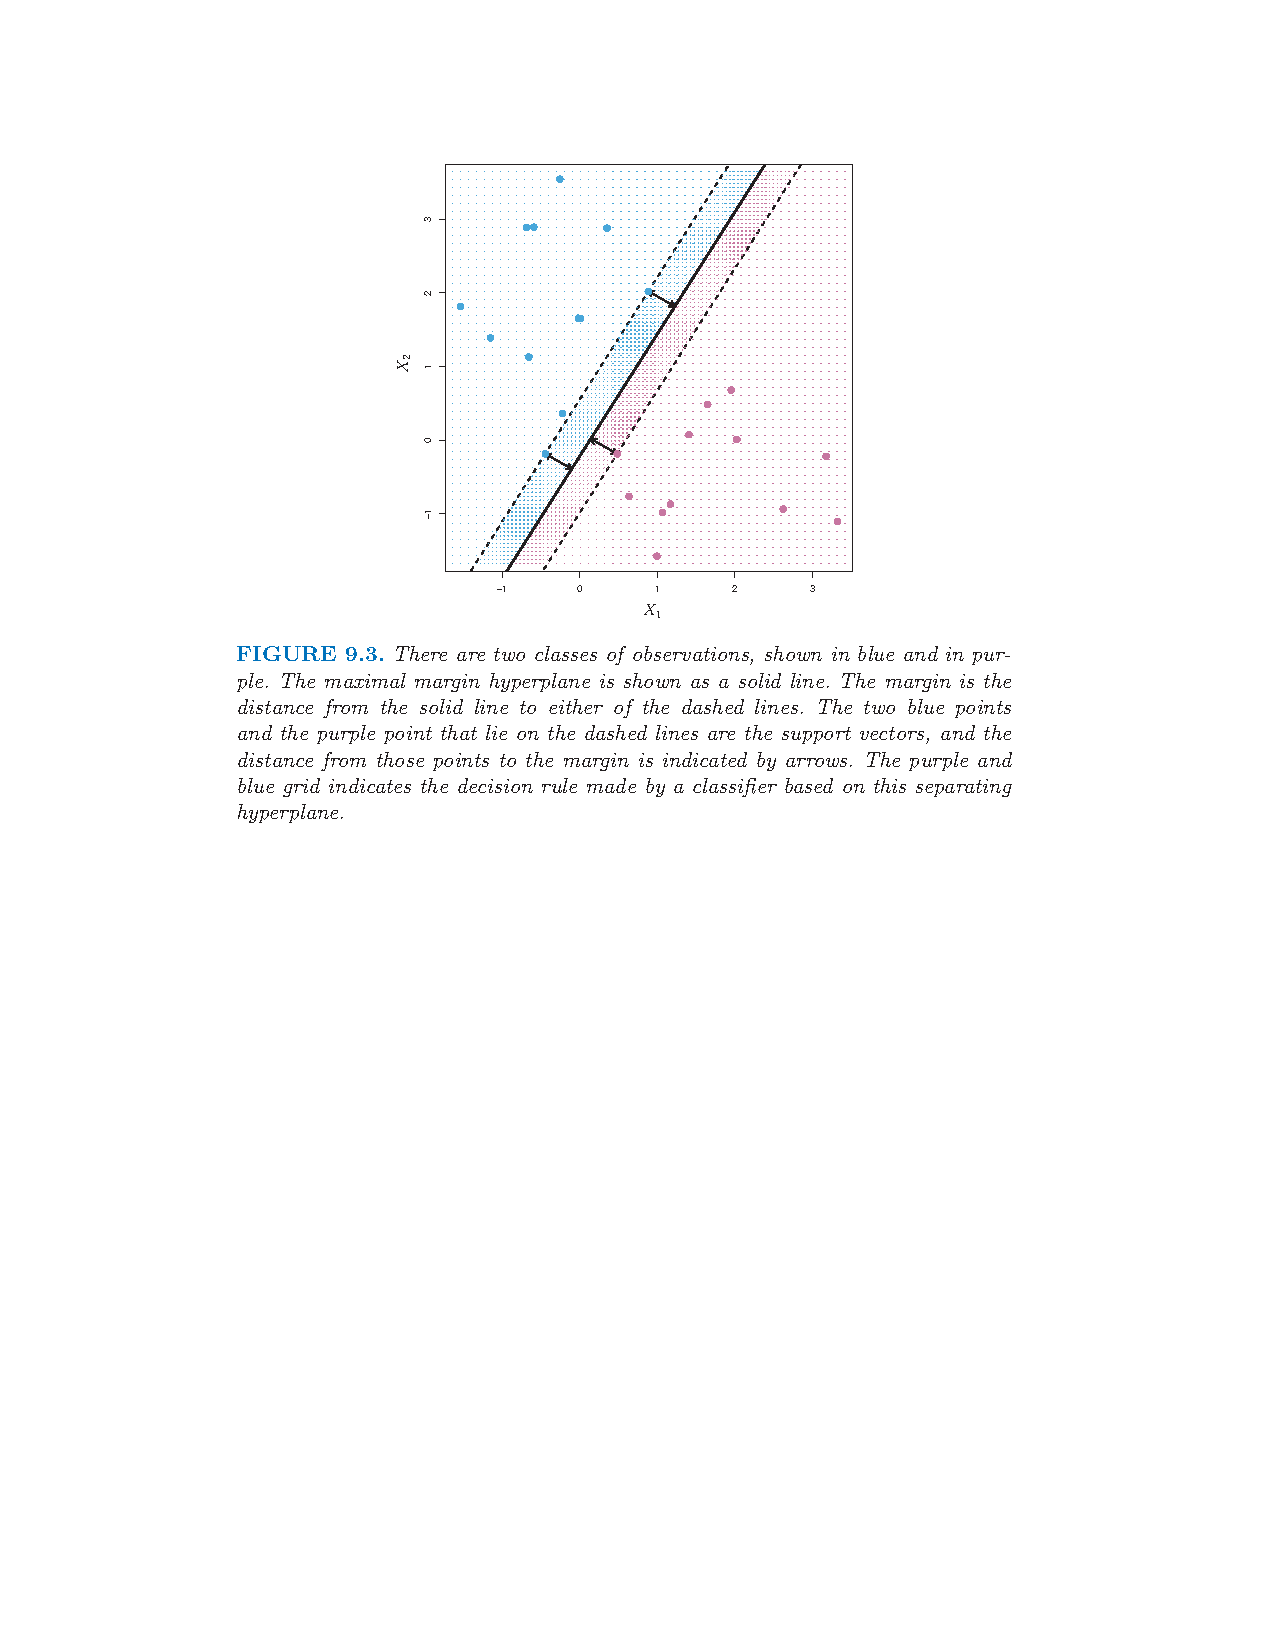
\includegraphics{StatLearningMarginPage357.pdf}
\end{center}

The goal is to maximize the margin around the separating hyperplane. This optimization turns out to be not that hard if you are in multivariable calculus \smiley{} but if you are in algebra, trig, or single-variable calculus, it is very hard. Fortunately, python is going to do the work for us!

\end{document}
